% !TEX TS-program = xelatex
% !TEX encoding = UTF-8

\documentclass[aspectratio=169]{beamer}
\usetheme{hfut-sx}

\usepackage{amsmath,amsfonts,amssymb}
\usepackage{multirow}
\usepackage{booktabs}
\usepackage{layout}
\usepackage{minted}
\usepackage[natbib=true]{biblatex}
\addbibresource{ref.bib}

\setbeamertemplate{frametitle continuation}[from second]

\AtBeginSection[]
{
  \begin{frame}{目录}
    \tableofcontents[currentsection]
  \end{frame}
}

\newcommand{\BibTeX}{\textsc{Bib}\TeX{}}
\newcommand{\BibLaTeX}{\textsc{Bib}\LaTeX{}}
\newcommand{\Beamer}{\textsc{Beamer}}
\newcommand{\enableindent}{\setlength{\parskip}{6pt}\setlength{\parindent}{2em}}
% algorithm
\usepackage{algorithm}
\usepackage{algorithmicx,algpseudocode}
\floatname{algorithm}{算法}

\title{《Linux 程序设计》课程大作业汇报}
\subtitle{及成果展示}
\author{徐启明 李文骏 胡雨牧 郑誉}
\institute{合肥工业大学}
\date{\today}

\begin{document}

\begin{frame}
    \maketitle
\end{frame}

\begin{frame}{目录}
    \tableofcontents
\end{frame}

\section{问题分析}

\begin{frame}[fragile]{问题目标}
    假设 $a>0$,求解如下问题 (\ref{problem}) 的最优解:

    \begin{equation}
        \min_{x\in\mathbb{R}}\frac{a}{2}x^2+dx+\sum^{m}_{i=1}\max(0,b_ix+c_i)\label{problem}
    \end{equation}

    \framebreak
\end{frame}

\begin{frame}[fragile]{问题转换}
    要求解问题 (\ref{problem}),即求解如下问题 (\ref{fx}) 的最优解:

    \begin{align}
        f(x)
         & =\frac{a}{2}x^2+dx+\sum^{m}_{i=1}\max(0,b_ix+c_i)\nonumber           \\
         & =\frac{a}{2}x^2+dx+\sum_{i\in I(b_ix+c_i)}\max(0,b_ix+c_i)\label{fx}
    \end{align}

    其中 $I(b_ix+c_i)=\{b_ix+c_i\ge0\}$
\end{frame}

\begin{frame}[fragile,allowframebreaks]{次梯度函数}
    要求解问题 (\ref{fx}),我们可以对问题 (\ref{fx}) 求次梯度函数:

    \begin{align}
        g(x)
         & =\partial f(x)\nonumber                    \\
         & =ax+d+\sum_{i\in I(b_ix+c_i)}b_i\label{gx}
    \end{align}

    根据图 (\ref{SubGradient}) 不难看出,$g(x)$ 是由如下断点集合分割的一个分段函数:

    \begin{equation}
        x=\{x_i|x_i=-\frac{c_i}{b_i},i=1\dots m\}\nonumber
    \end{equation}

    \framebreak

    次梯度函数 $g(x)$ 图像如图所示:

    \begin{figure}[htb]
        \centering
        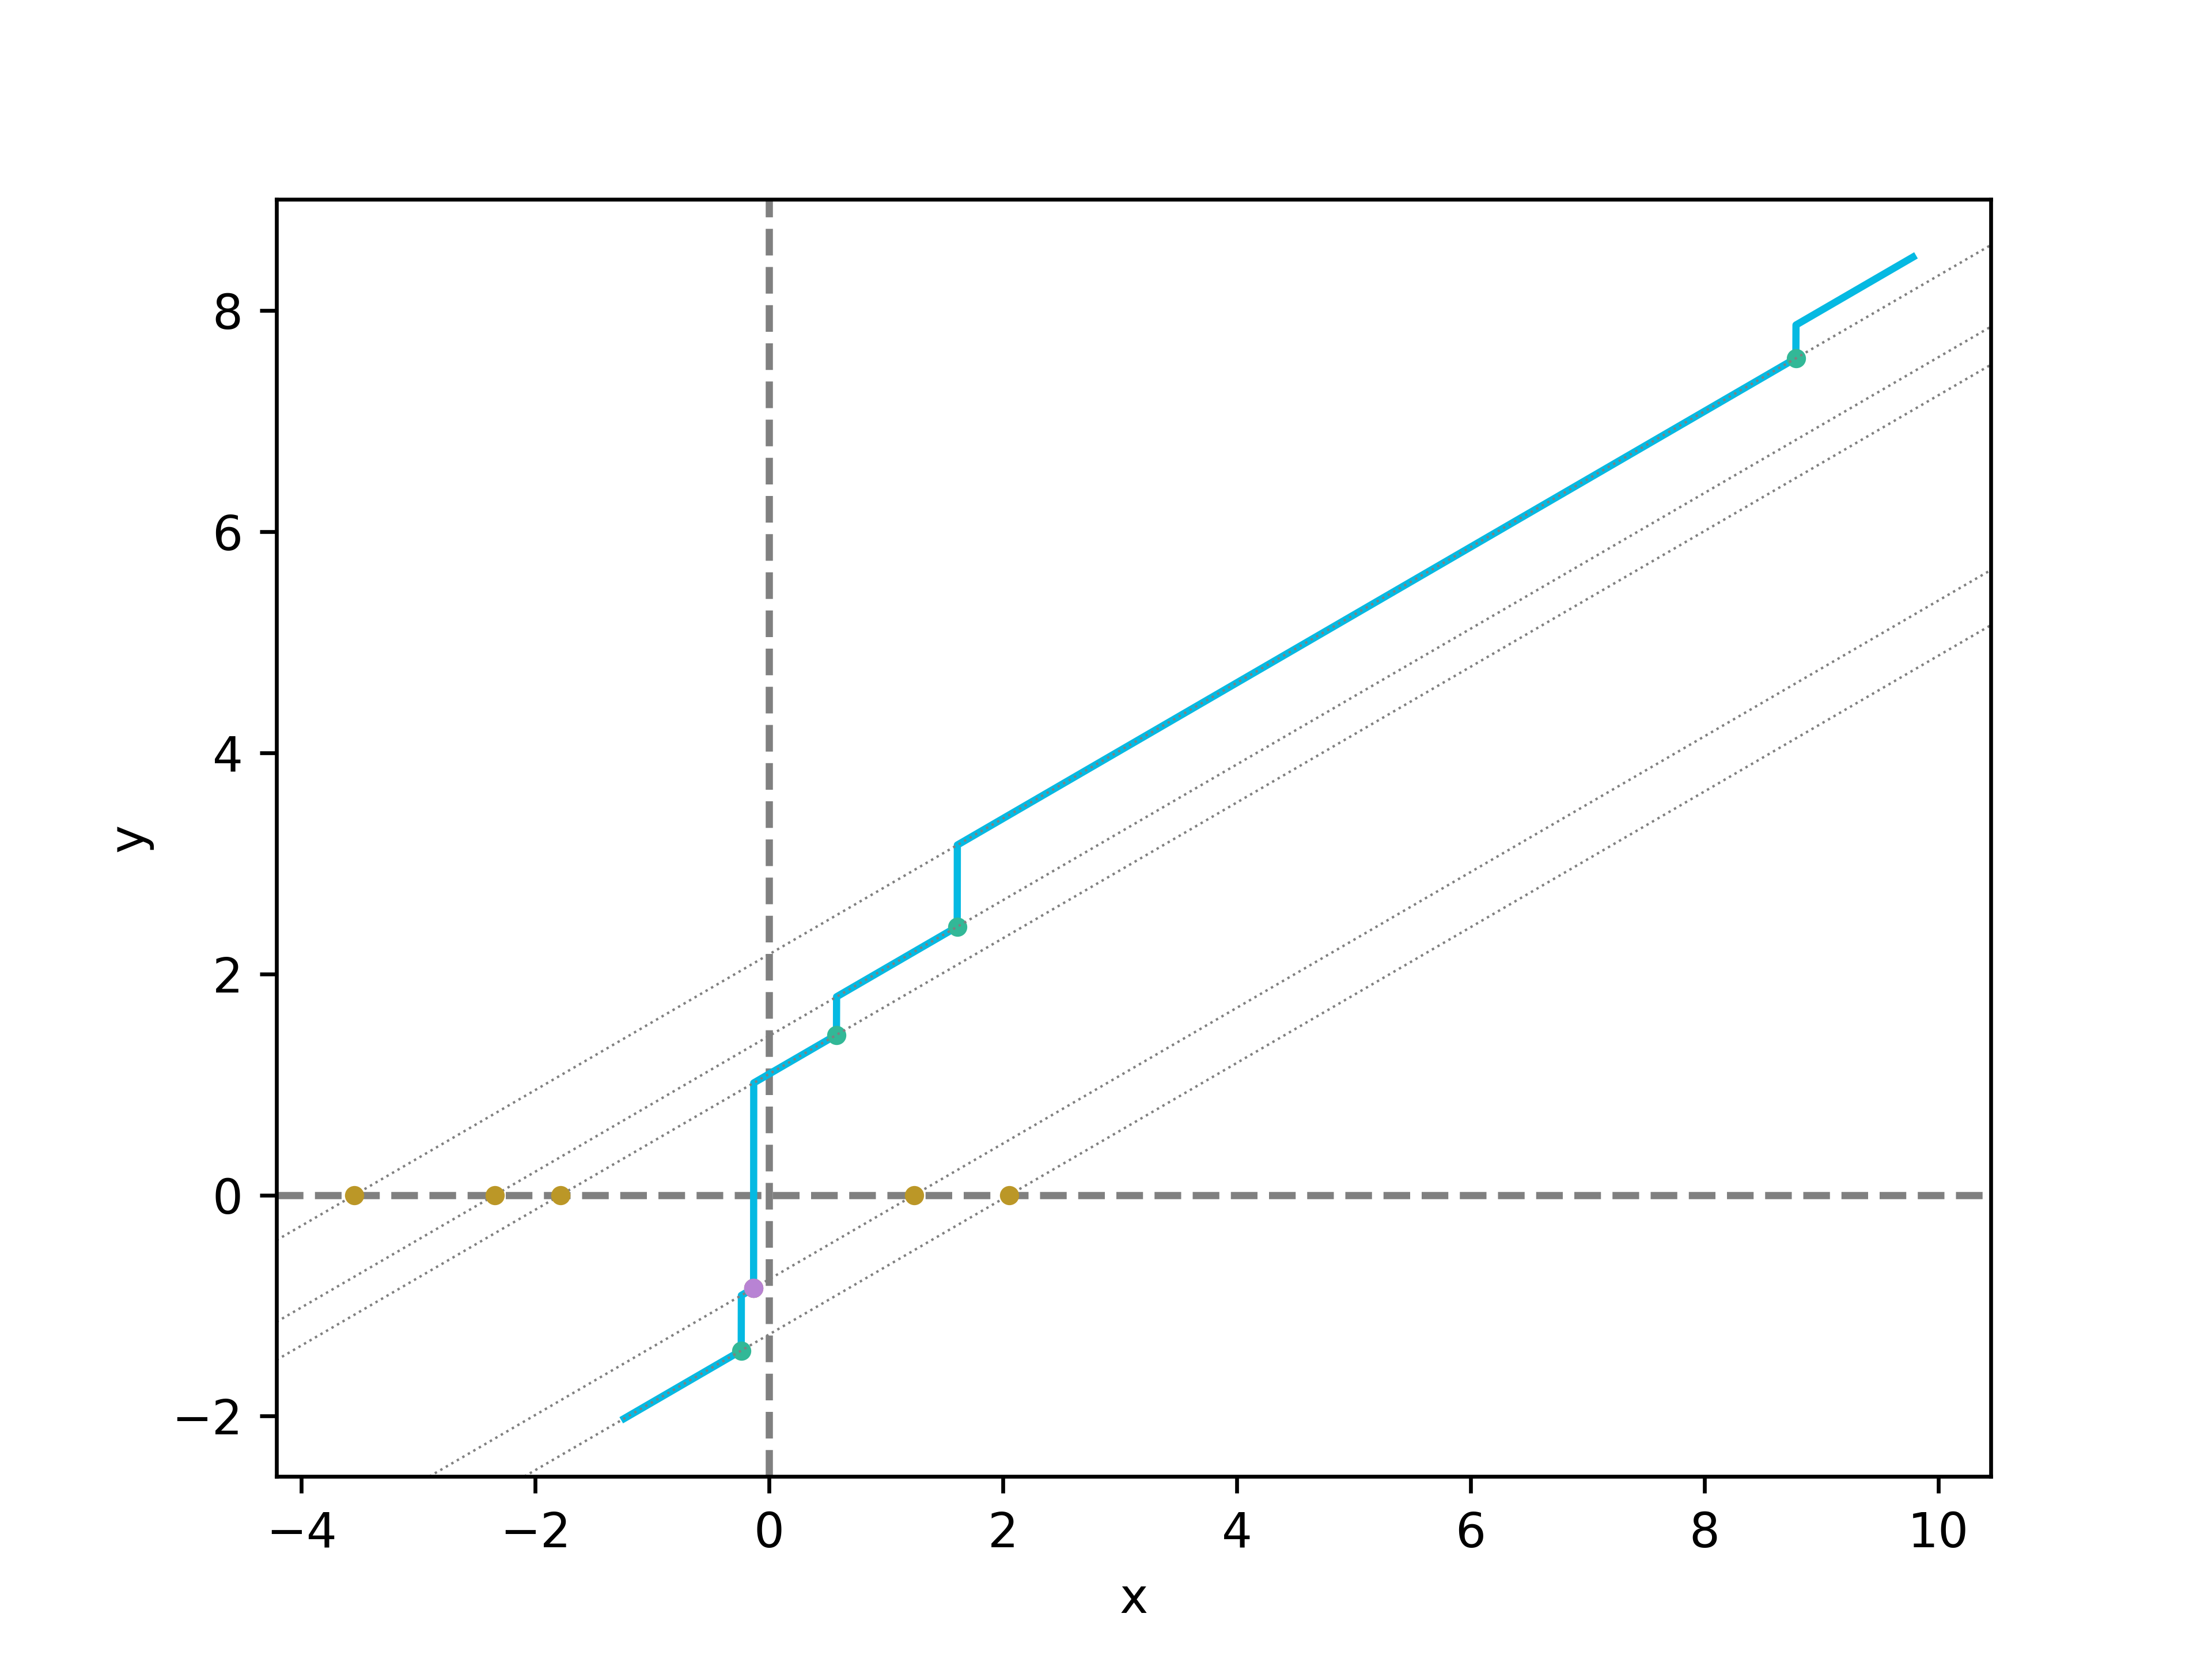
\includegraphics[width=0.33\textwidth]{images/SubGradient.png}
        \caption{次梯度函数图像}
        \label{SubGradient}
    \end{figure}
\end{frame}

\begin{frame}[fragile]{问题目标}
    基于前文所述,要求解原问题 (\ref{problem}),即求解一 $x^*$ 使得 $x^*\in \mathbb{R}\text{且}0\in g(x^*)$。
\end{frame}

\section{算法设计}

\begin{frame}[fragile,allowframebreaks]{算法设计}
    我们设计了两种算法来求解问题 (\ref{problem}),分别是:

    \begin{itemize}
        \item 基于参考文献 \cite{10.1016/j.patcog.2017.02.006} 的随机化中值查找算法:该算法的核心思想是通过将断点分割为 $L$ 集合和 $G$ 集合,其中 $L$ 集合中储存小于当前断点的断点下标,$G$ 集合中储存大于当前断点的断点下标。在分割完成后,通过判断 $g(x)$ 的符号来确定如何求解原问题 (\ref{problem})。
        \item 基于参考文献 \cite{10.5555/1577069.1755859} 的排序后二分查找算法:该算法的核心思想是通过将断点进行从小到大的排序,而后使用二分法查找最终解。
    \end{itemize}

    \framebreak

    \enableindent

    在实现随机化中值查找算法,我们发现完全按照参考文献 \cite{10.1016/j.patcog.2017.02.006} 中算法三的伪代码进行编写并不能正确的完成问题的求解。通过排查算法中的相关问题,我们删去了通过前一次计算的 $g(x)$ 值来计算当前 $g(x)$ 值的相关部分,并使用直接求解 $g(x)$ 来代替前者。

    此外,我们还发现,如果完全使用程序求解的 $g(x)$ 值作为实际 $g(x)$ 值,那么就会出现一些偏差。这会导致断点对应的 $g(x)$ 值或在上方、或在下方,并且所求的解也存在严重偏差。如图 (\ref{Error}) 所示,断点所在位置存在偏差,两个算法的解均不正确。

    \framebreak

    \begin{figure}[htb]
        \centering
        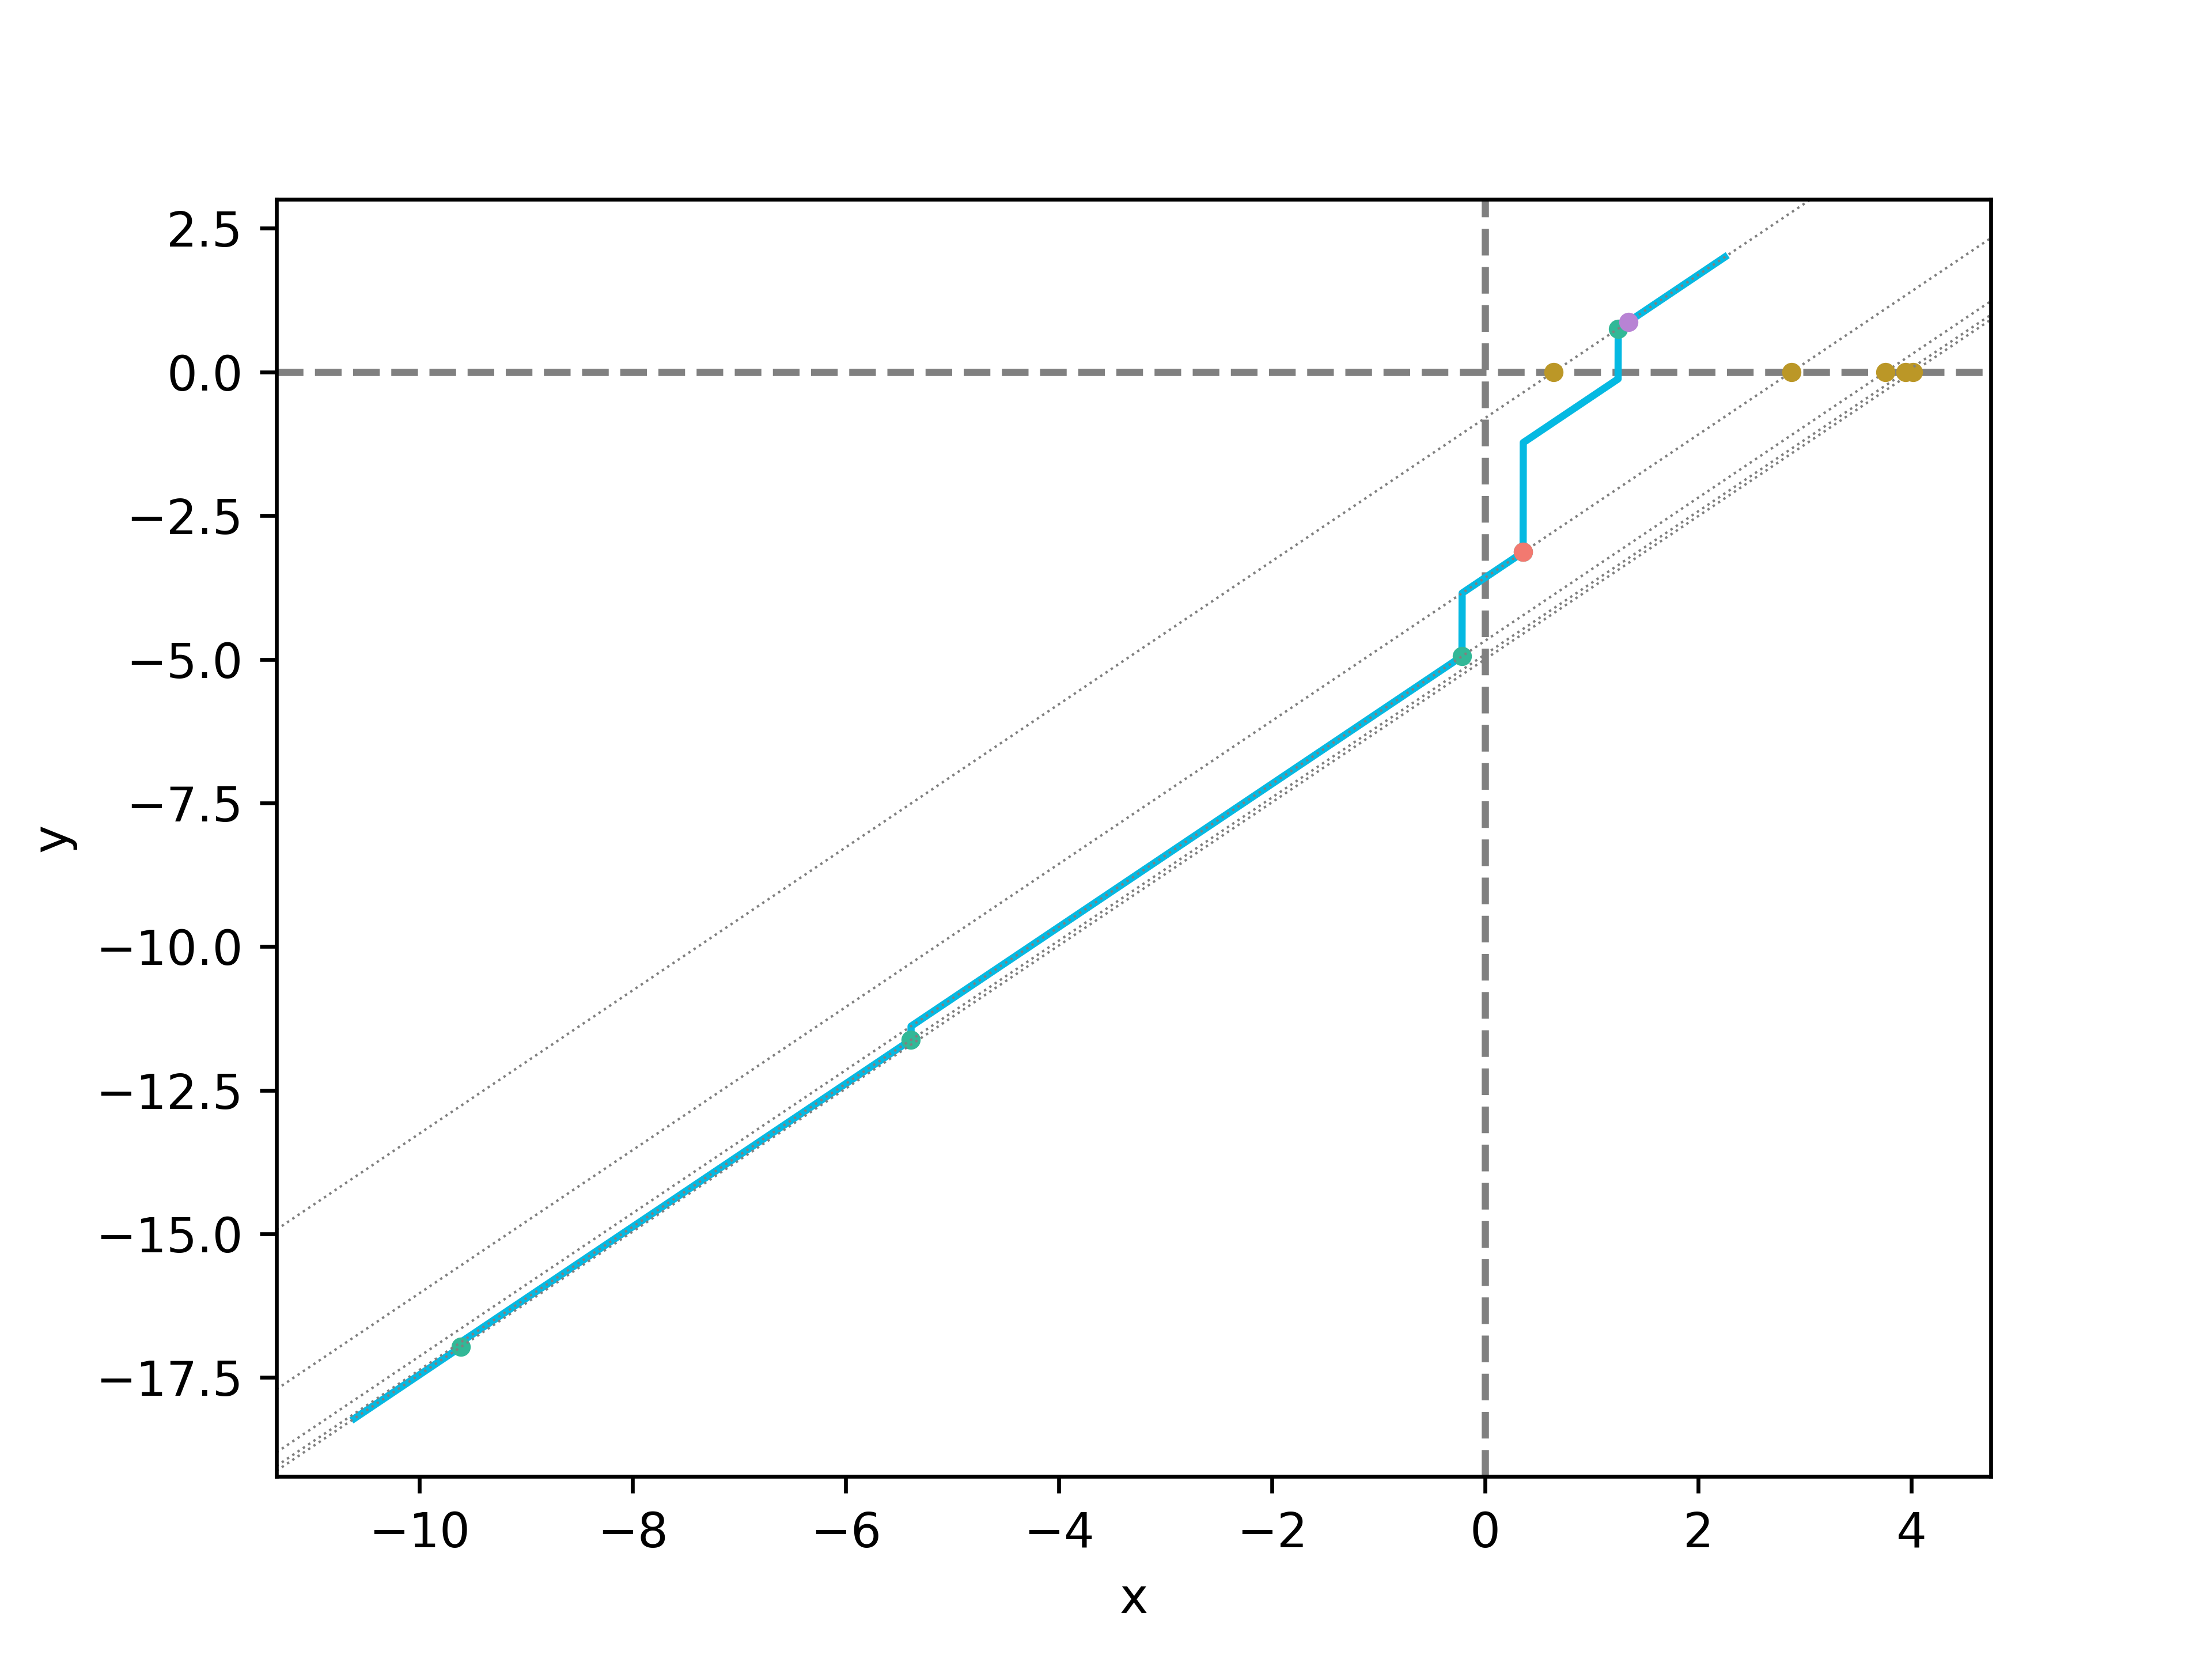
\includegraphics[width=0.5\textwidth]{images/Error.png}
        \caption{错误的次梯度函数图像}
        \label{Error}
    \end{figure}
\end{frame}

\begin{frame}[fragile]{算法测试}
    \enableindent

    给定 $a=1.5,d=1,b=[1;1.2;−0.9],c=[0.1;−1.4;−1.2]$,使用上述两个算法求解结果如图所示(紫色点即为求解结果):

    \begin{figure}[htb]
        \centering
        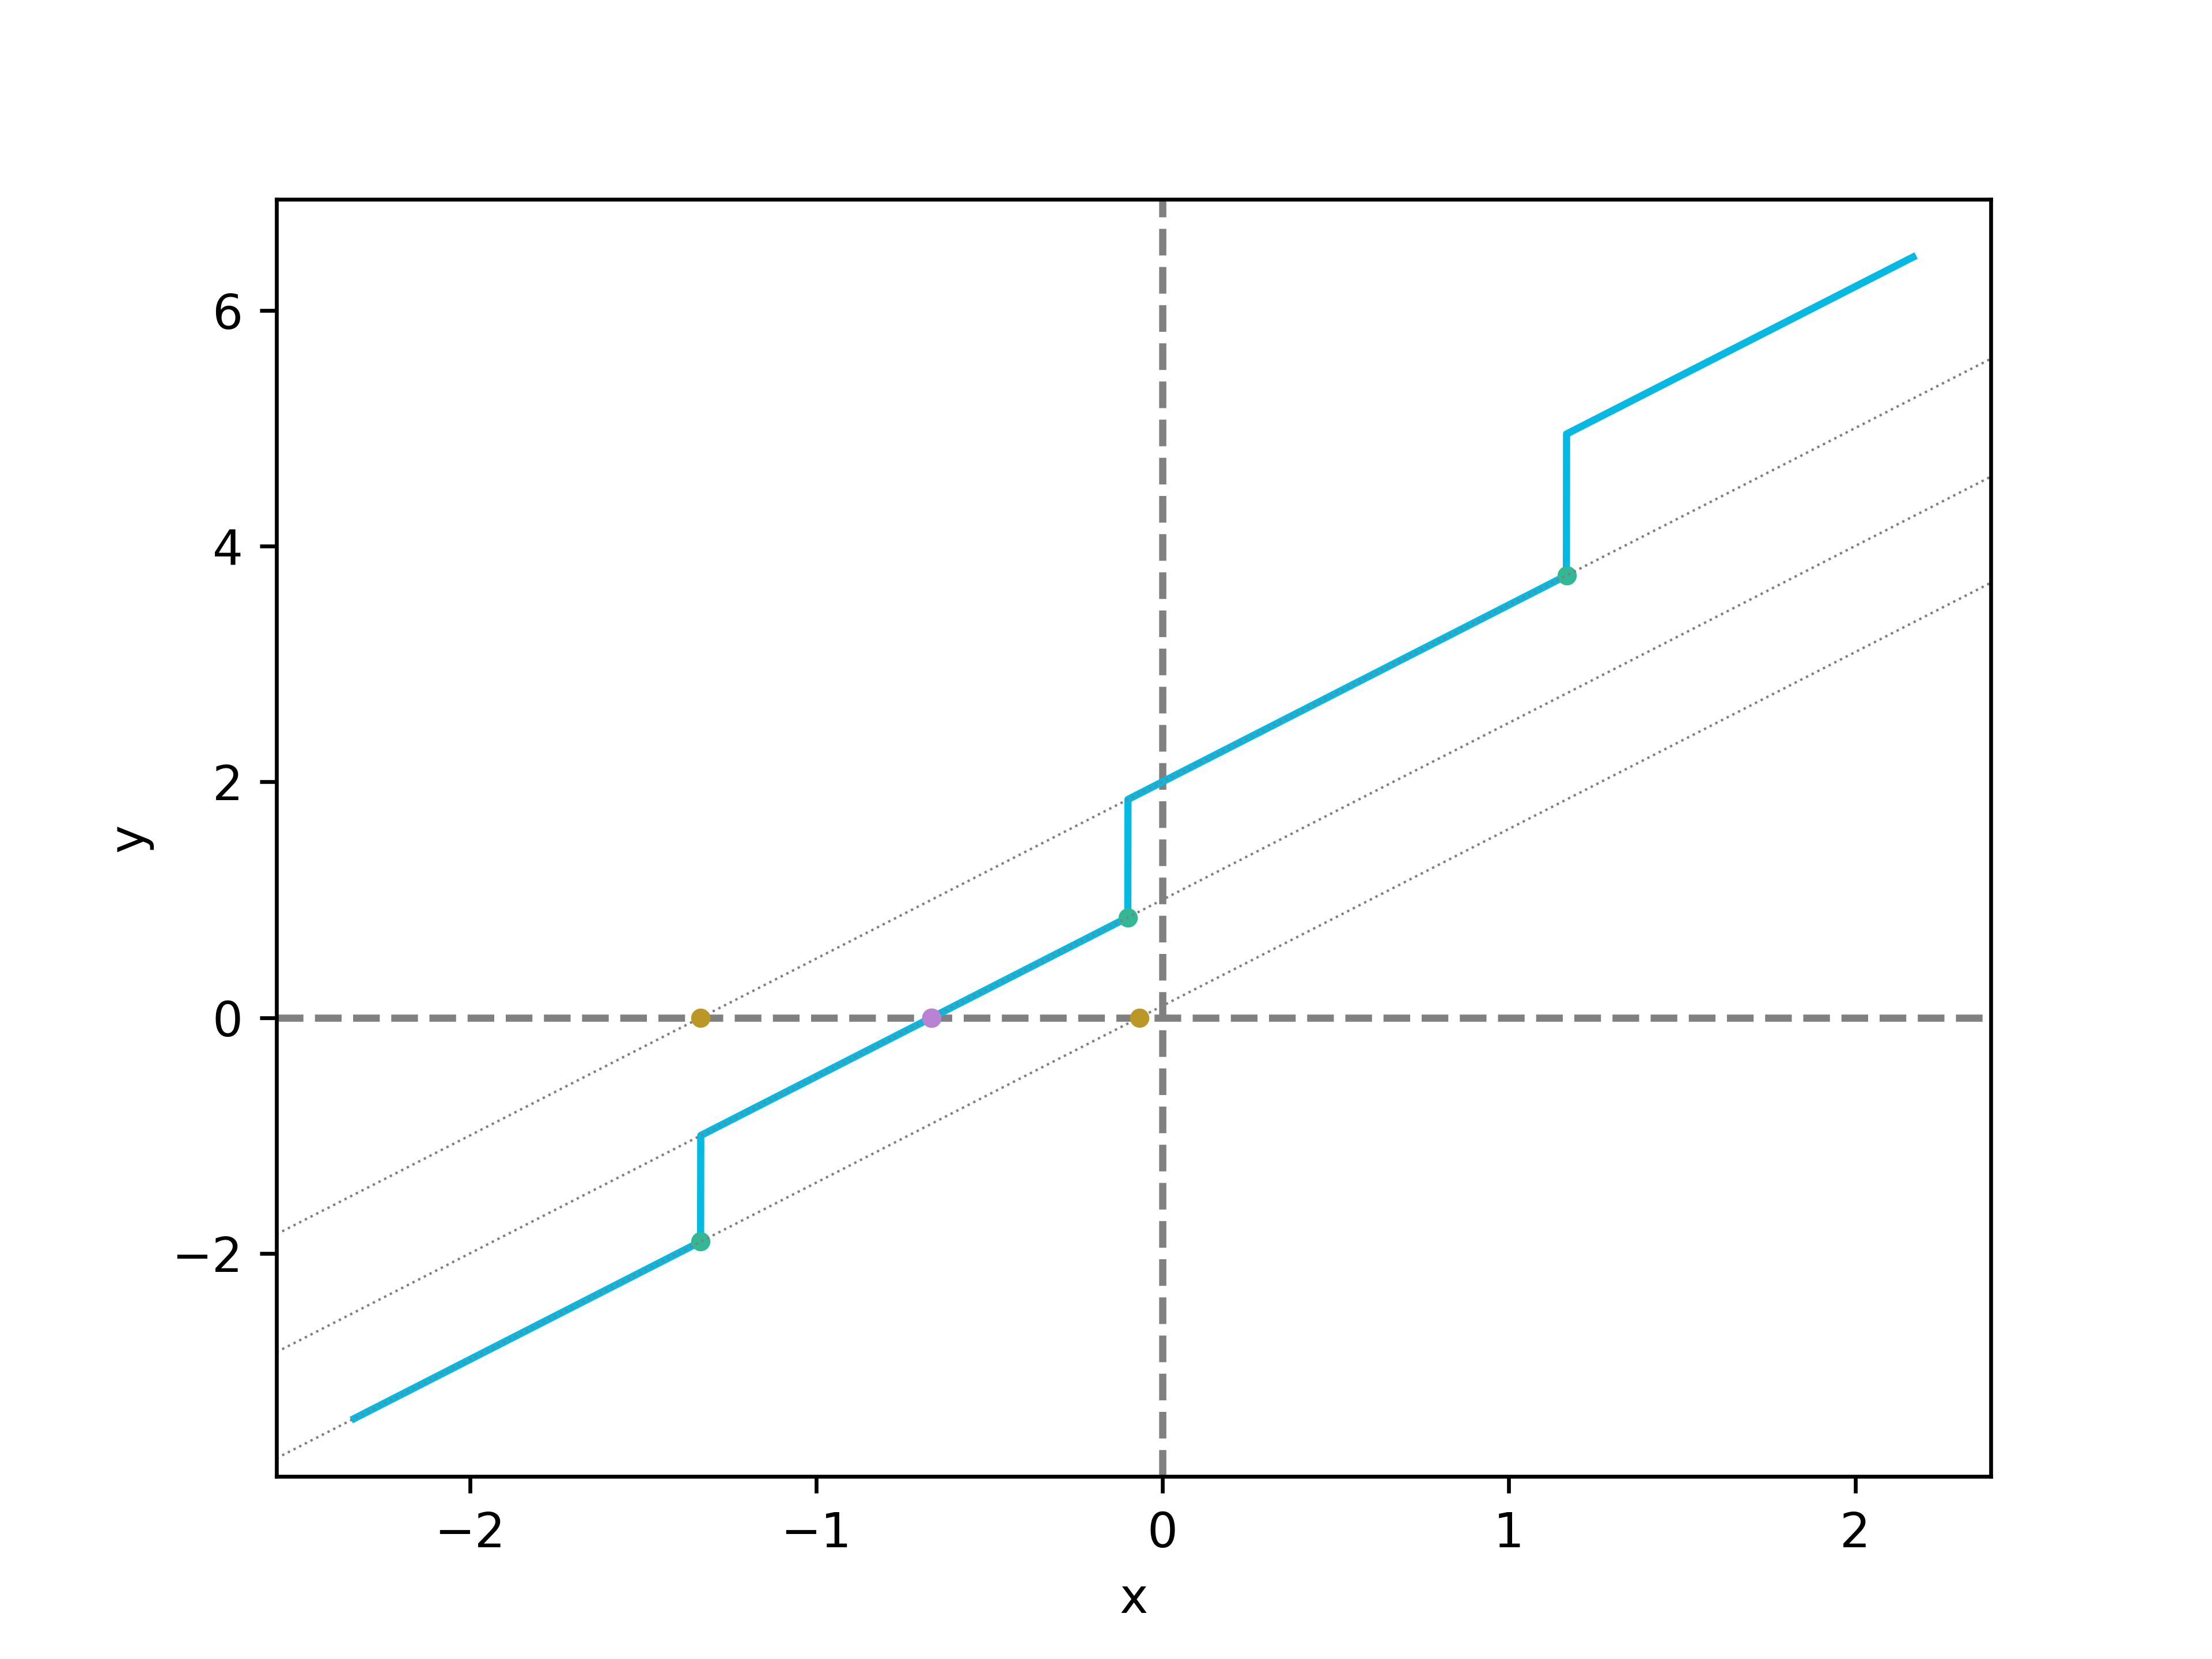
\includegraphics[width=0.33\textwidth]{images/Answer.png}
        \caption{求解结果}
        \label{Answer}
    \end{figure}
\end{frame}

\section{性能比较}

\begin{frame}[fragile]{性能比较}
    在性能比较时,我们令 $a,d,b,c$ 依照如下分布:

    \begin{align}
        a & =|randn(1)|\nonumber  \\
        d & =randn(1)\nonumber    \\
        b & =randn(m, 1)\nonumber \\
        c & =randn(m, 1)\nonumber
    \end{align}
    并令 $m=10^2,10^3,10^4,10^5,10^6$
\end{frame}

\begin{frame}[fragile]{性能比较}
    \enableindent

    两个算法的性能比较如下图所示,其中橙色线为排序后二分查找算法;蓝色线为随机化中值查找算法;绿色线为两算法所耗时间的差值

    \begin{figure}[htb]
        \centering
        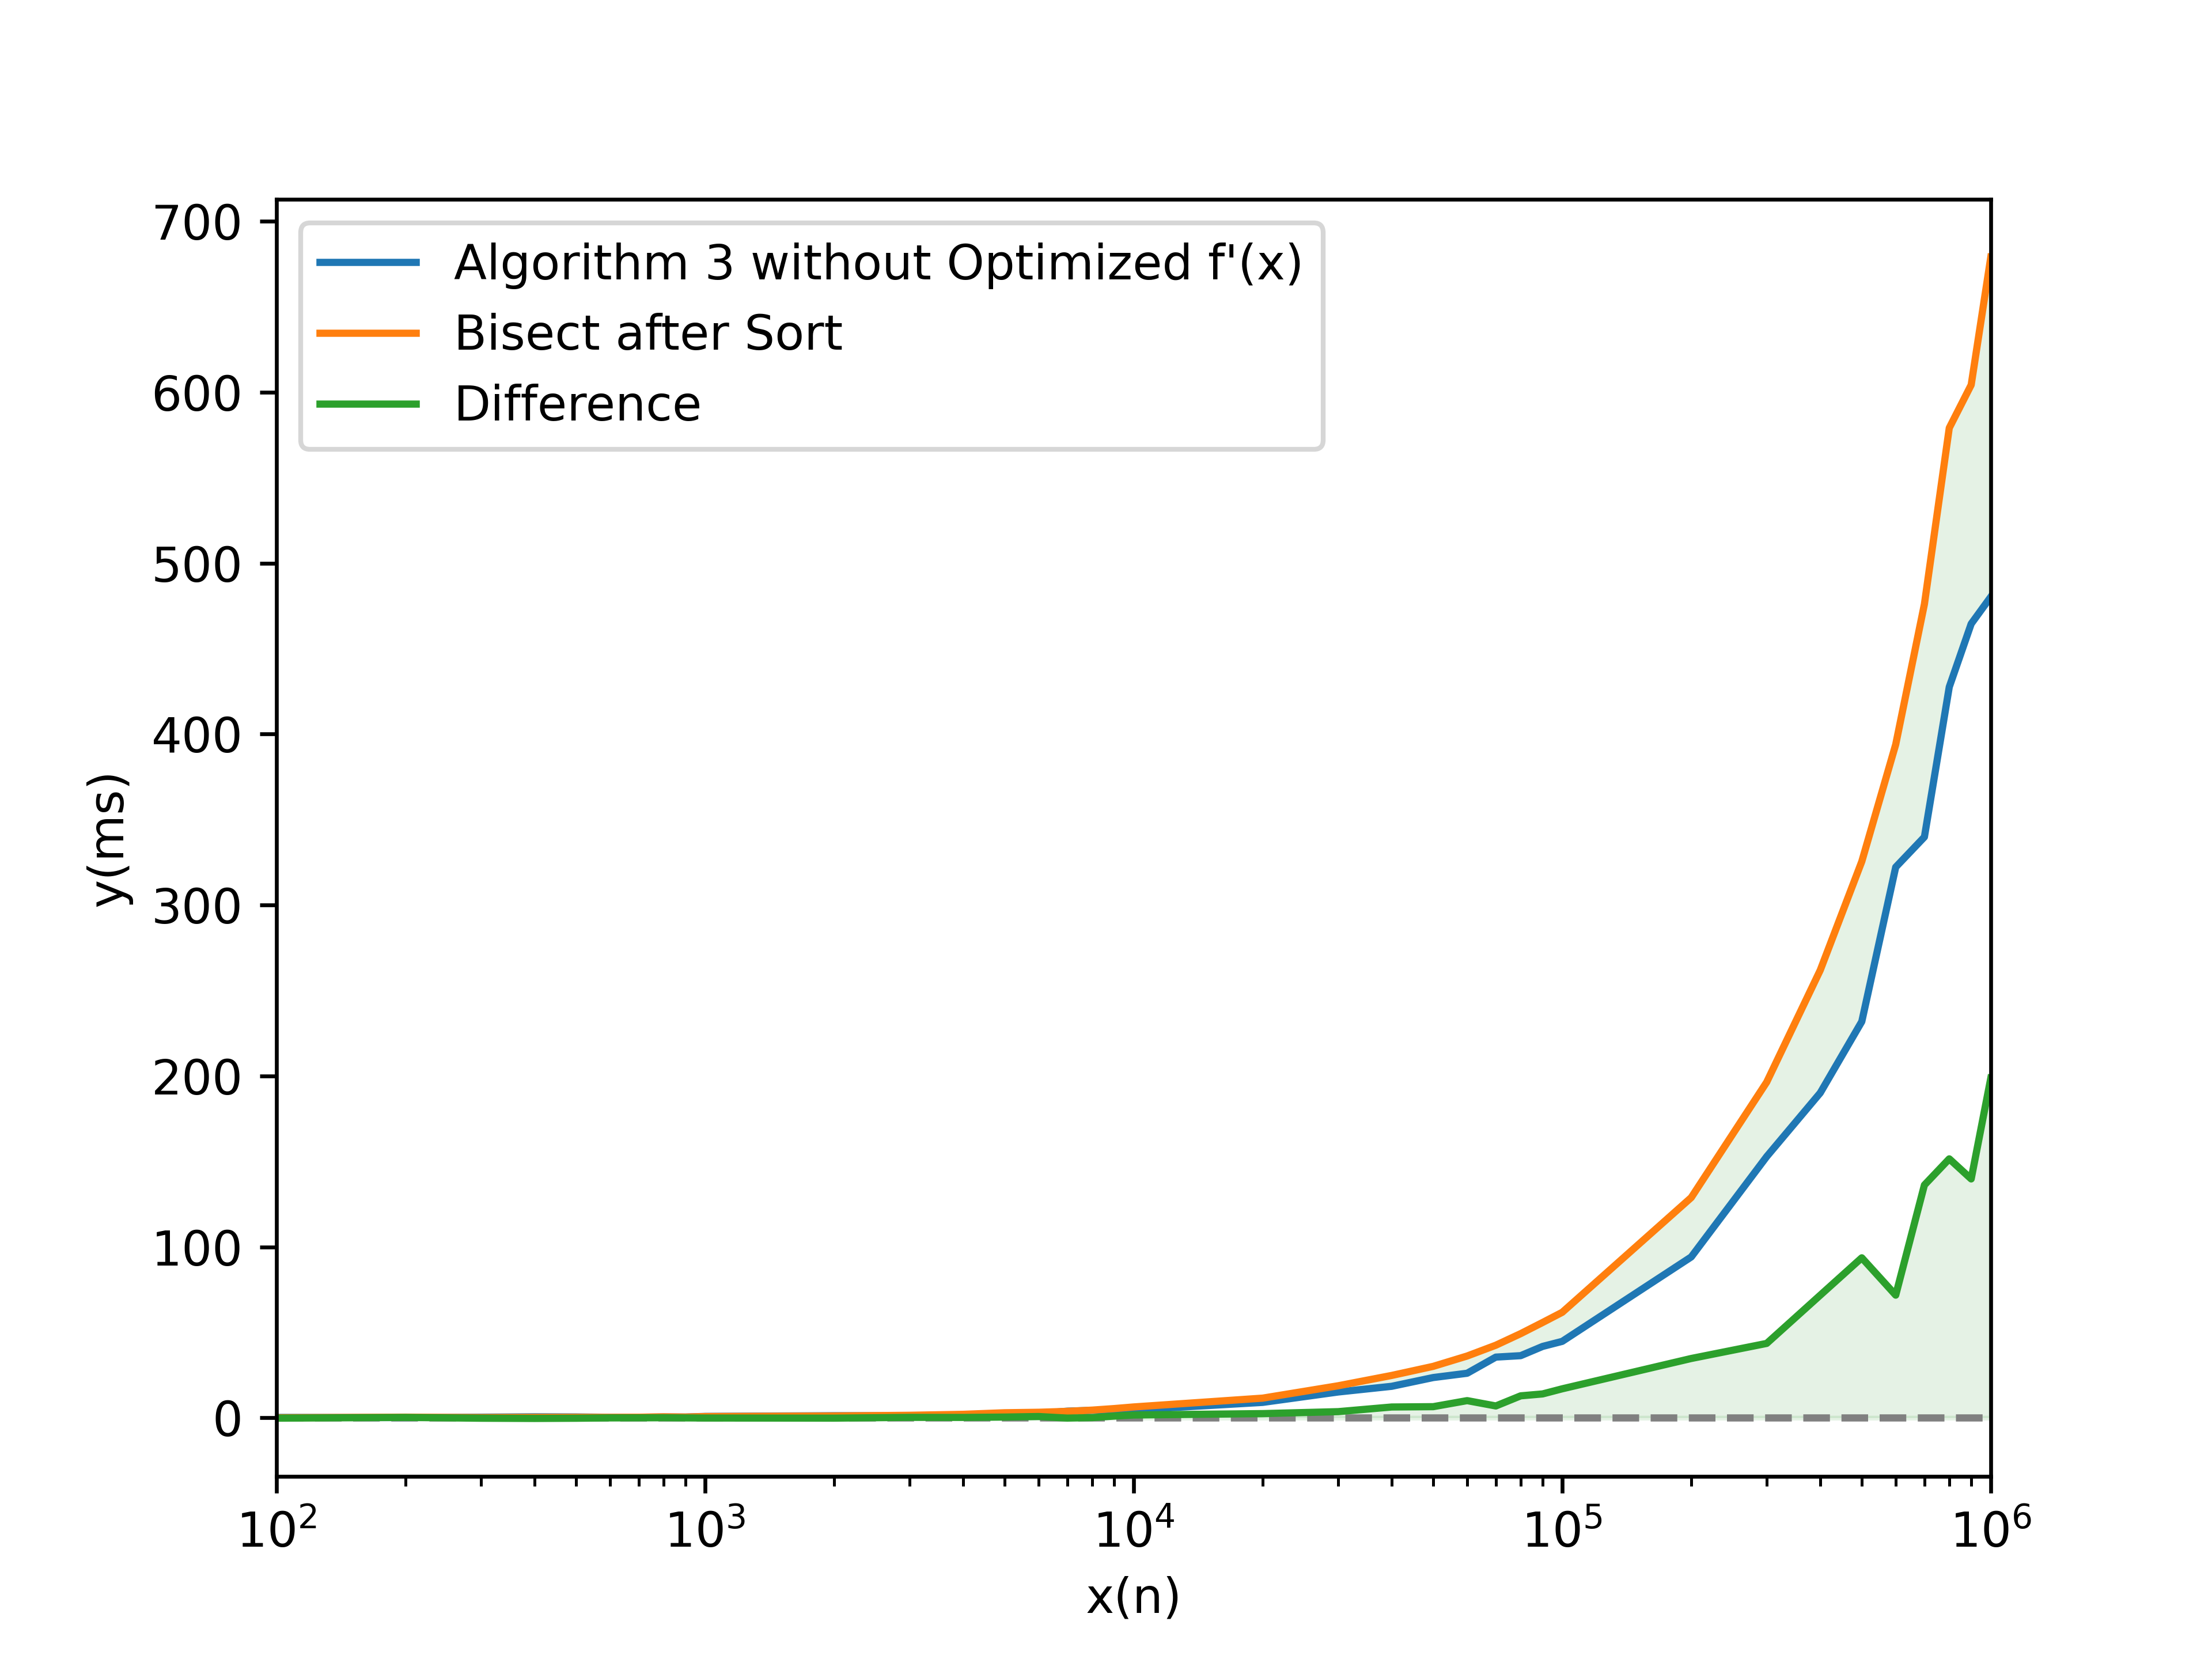
\includegraphics[width=0.33\textwidth]{images/Compare.png}
        \caption{性能比较}
        \label{Compare}
    \end{figure}
\end{frame}

\section{源程序}

\begin{frame}[fragile]{源程序}
    源程序已经上传至 GitHub,链接分别如下:

    \begin{itemize}
        \item Python 语言编写的绘图程序:https://github.com/xqm32/unix-report-python
        \item C 语言实现的算法程序:https://github.com/xqm32/unix-report
    \end{itemize}
\end{frame}

\begin{frame}[fragile]{小组分工}
    本组成员分工如下:

    \begin{itemize}
        \item 徐启明:Python 算法原型实现
        \item 李文骏:C 语言算法具体实现
        \item 胡雨牧:Beamer 撰写、算法性能分析及绘图
        \item 郑 誉:测试脚本实现、算法绘图
    \end{itemize}
\end{frame}

\begin{frame}[allowframebreaks]
    \frametitle{参考文献}
    {
        \tiny
        \nocite{*}
        \printbibliography[heading=none]
    }
\end{frame}

\end{document}
